\section{Systemet i helhet}
Robeten byggs på en trehjulig plattform(CarpetRover). På plattformen kommer tre enheter att monteras:
\begin{itemize}
        \item Kommunikationsenhet
        \item Sensorenhet
        \item Styrenhet
Varje enhet kommer styras av en egen AVR-processor.
\subsection{Kommunikation}
De tre enheterna måste kunna kommunicera med varandra, här förslås en I2C-buss och ett system med flera UART.

\subsubsection{I2C}

\end{itemize}
\begin{center}
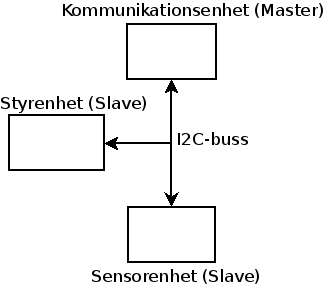
\includegraphics[scale=0.7]{delsystem_i2c.png}
\end{center}
De olika enheterna kommer att kommunicera över en I2C-buss där kommunikationsenheten är master och de andra två enheterna är slave,
detta är för att den mesta kommunikationen kommer att ske genom kommunkationsenheten.

\subsubsection{UART}

\begin{center}
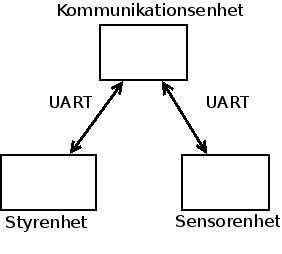
\includegraphics[scale=0.7]{delsystem_uart.png}
\end{center}
De olika enheterna kommer att kommunicera med de i processorerna inbyggda UART-portarna. 
Då dessa redan finns i processorerna blir de lättare att implementera. Det finns dock en nackdel, UART är en 
punkt till punkt kommunikation och då det är tre enheter som måste kommunicera med varandra måste minst en enhet
ha två UART-portar, men processorerna har bara en inbyggd UART-port. Detta går att lösa genom att omvandla en av de generella 
IO-portarna på processorerna till en UART med hjälp av mjukvara. 
Det räcker med att kommunikationsenhten har en extra UART om all kommunikation sker genom den enheten.

\subsection{Uppgraderbarhet}
Ett tydligt kommunikationsprotokoll mellan enheterna kommer att användas så att det är lätt att modifiera enheter.
Om en I2C-buss används blir det lättare at lägga till och byta ut enheter då I2C kan ses som en standardbuss.
Om istället UART används som kommunikation blir det svårare att lägga till nya enheter då flera UART-portar måste implementeras.
Att byta ut eller uppgradera en enhet blir dock lika enkelt med en UART som med en I2C.

PC-mjukavaran kommer att skicka och ta emot data från kommunikationsenheten via blåtand.
Mjukvaran kommer att använda ett tydligt protokoll vilket gör det möjligt att utveckla egen mjukvara eller uppgradera den befintliga mjukvaran.
